\documentclass[12pt,]{article}
\usepackage[left=1in,top=1in,right=1in,bottom=1in]{geometry}
\newcommand*{\authorfont}{\fontfamily{phv}\selectfont}
\usepackage[]{mathpazo}


  \usepackage[T1]{fontenc}
  \usepackage[utf8]{inputenc}




\usepackage{abstract}
\renewcommand{\abstractname}{}    % clear the title
\renewcommand{\absnamepos}{empty} % originally center

\renewenvironment{abstract}
 {{%
    \setlength{\leftmargin}{0mm}
    \setlength{\rightmargin}{\leftmargin}%
  }%
  \relax}
 {\endlist}

\makeatletter
\def\@maketitle{%
  \newpage
%  \null
%  \vskip 2em%
%  \begin{center}%
  \let \footnote \thanks
    {\fontsize{18}{20}\selectfont\raggedright  \setlength{\parindent}{0pt} \@title \par}%
}
%\fi
\makeatother




\setcounter{secnumdepth}{0}

\usepackage{longtable,booktabs}

\usepackage{graphicx,grffile}
\makeatletter
\def\maxwidth{\ifdim\Gin@nat@width>\linewidth\linewidth\else\Gin@nat@width\fi}
\def\maxheight{\ifdim\Gin@nat@height>\textheight\textheight\else\Gin@nat@height\fi}
\makeatother
% Scale images if necessary, so that they will not overflow the page
% margins by default, and it is still possible to overwrite the defaults
% using explicit options in \includegraphics[width, height, ...]{}
\setkeys{Gin}{width=\maxwidth,height=\maxheight,keepaspectratio}


\title{CS 230 Project: Preanalysis \thanks{Code and data available at: github.com/rossdahlke/cs\_230\_project}  }



\author{\Large Ross Dahlke
(\href{mailto:rdahlke@stanford.edu}{\nolinkurl{rdahlke@stanford.edu}})\vspace{0.05in} \newline\normalsize\emph{}  }


\date{}

\usepackage{titlesec}

\titleformat*{\section}{\normalsize\bfseries}
\titleformat*{\subsection}{\normalsize\itshape}
\titleformat*{\subsubsection}{\normalsize\itshape}
\titleformat*{\paragraph}{\normalsize\itshape}
\titleformat*{\subparagraph}{\normalsize\itshape}





\newtheorem{hypothesis}{Hypothesis}
\usepackage{setspace}


% set default figure placement to htbp
\makeatletter
\def\fps@figure{htbp}
\makeatother


% move the hyperref stuff down here, after header-includes, to allow for - \usepackage{hyperref}

\makeatletter
\@ifpackageloaded{hyperref}{}{%
\ifxetex
  \PassOptionsToPackage{hyphens}{url}\usepackage[setpagesize=false, % page size defined by xetex
              unicode=false, % unicode breaks when used with xetex
              xetex]{hyperref}
\else
  \PassOptionsToPackage{hyphens}{url}\usepackage[draft,unicode=true]{hyperref}
\fi
}

\@ifpackageloaded{color}{
    \PassOptionsToPackage{usenames,dvipsnames}{color}
}{%
    \usepackage[usenames,dvipsnames]{color}
}
\makeatother
\hypersetup{breaklinks=true,
            bookmarks=true,
            pdfauthor={Ross Dahlke
(\href{mailto:rdahlke@stanford.edu}{\nolinkurl{rdahlke@stanford.edu}}) ()},
             pdfkeywords = {},  
            pdftitle={CS 230 Project: Preanalysis},
            colorlinks=true,
            citecolor=blue,
            urlcolor=blue,
            linkcolor=magenta,
            pdfborder={0 0 0}}
\urlstyle{same}  % don't use monospace font for urls

% Add an option for endnotes. -----


% add tightlist ----------
\providecommand{\tightlist}{%
\setlength{\itemsep}{0pt}\setlength{\parskip}{0pt}}

% add some other packages ----------

% \usepackage{multicol}
% This should regulate where figures float
% See: https://tex.stackexchange.com/questions/2275/keeping-tables-figures-close-to-where-they-are-mentioned
\usepackage[section]{placeins}


\begin{document}
	
% \pagenumbering{arabic}% resets `page` counter to 1 
%
% \maketitle

{% \usefont{T1}{pnc}{m}{n}
\setlength{\parindent}{0pt}
\thispagestyle{plain}
{\fontsize{18}{20}\selectfont\raggedright 
\maketitle  % title \par  

}

{
   \vskip 13.5pt\relax \normalsize\fontsize{11}{12} 
\textbf{\authorfont Ross Dahlke
(\href{mailto:rdahlke@stanford.edu}{\nolinkurl{rdahlke@stanford.edu}})} \hskip 15pt \emph{\small }   

}

}






\vskip -8.5pt


 % removetitleabstract

\noindent \doublespacing 

\hypertarget{the-main-purpose-of-this-document-is-to-analyze-the-results-of-the-dps-in-order-to-determine-which-questions-should-be-used-in-the-analysis.}{%
\section{The main purpose of this document is to analyze the results of
the DPs in order to determine which questions should be used in the
analysis.}\label{the-main-purpose-of-this-document-is-to-analyze-the-results-of-the-dps-in-order-to-determine-which-questions-should-be-used-in-the-analysis.}}

I will calculate on which issues opinions change the most, or if I can
even use an average of all of the questions.

\hypertarget{ghana}{%
\subsection{Ghana}\label{ghana}}

\hypertarget{food-safety-and-livelihood}{%
\subsubsection{Food Safety and
Livelihood}\label{food-safety-and-livelihood}}

The following questions have to do with food safety and livelihood:

\begin{itemize}
\tightlist
\item
  q3
\item
  q12
\item
  q14
\end{itemize}

Looks like the average delta is the same across all, so we can use all
the groups.

\begin{longtable}[]{@{}rrrr@{}}
\toprule
delta\_q3 & delta\_q12 & delta\_q14 & delta\_all\tabularnewline
\midrule
\endhead
0.5765451 & 0.5518941 & 0.5632125 & 0.5638839\tabularnewline
\bottomrule
\end{longtable}

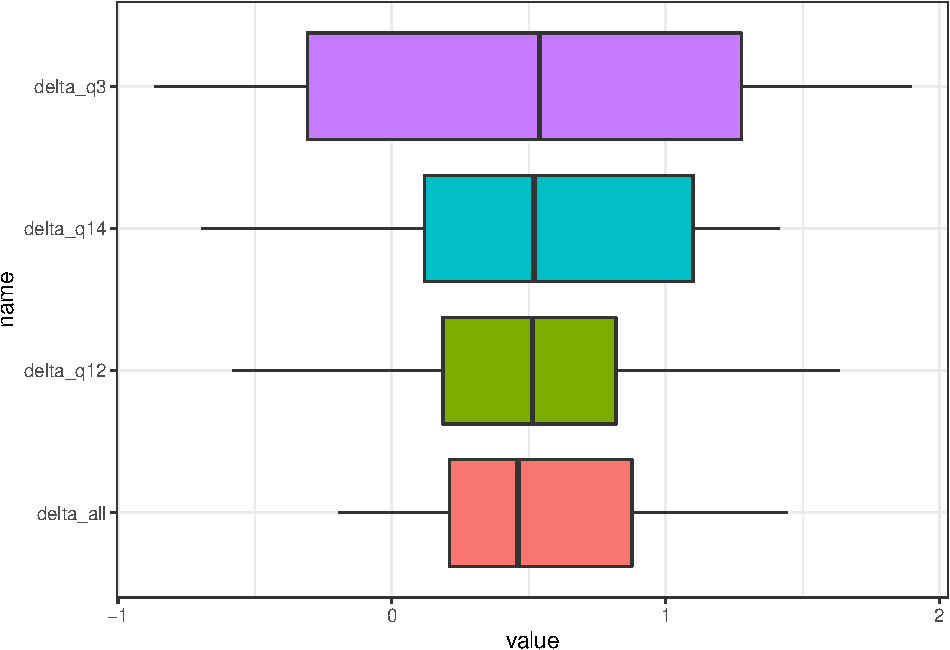
\includegraphics{preanalysis_files/figure-latex/unnamed-chunk-7-1.pdf}

\hypertarget{water-policy}{%
\subsection{Water policy}\label{water-policy}}

The following questions have to do with food safety and livelihood:

\begin{itemize}
\tightlist
\item
  q5
\item
  q20
\item
  q29
\item
  q33
\end{itemize}

The deltas aren't huge here. I'll keep all of the data.

\begin{longtable}[]{@{}rrrrr@{}}
\toprule
delta\_q5 & delta\_q20 & delta\_q29 & delta\_q33 &
delta\_all\tabularnewline
\midrule
\endhead
0.5324381 & 0.2628249 & 0.5400384 & 0.4743246 & 0.4524065\tabularnewline
\bottomrule
\end{longtable}

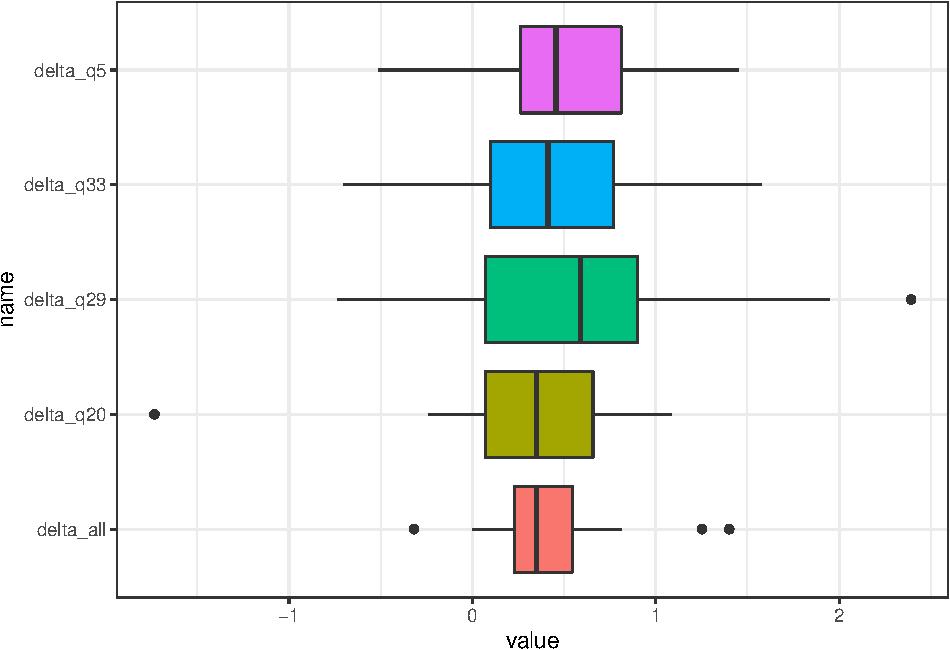
\includegraphics{preanalysis_files/figure-latex/unnamed-chunk-12-1.pdf}

\hypertarget{bududa}{%
\subsection{Bududa}\label{bududa}}

\hypertarget{land-management}{%
\subsection{Land Management}\label{land-management}}

\begin{itemize}
\tightlist
\item
  {[}28{]} ``x114\_planttrees\_protectriverbeds''\\
\item
  {[}29{]} ``x115\_riverchannels\_localgovernment''\\
\item
  {[}30{]} ``x116\_wetlands\_dryseason''\\
\item
  {[}31{]} ``x117\_riceschemes\_notinwetlands''\\
\item
  {[}32{]} ``x118\_communities\_maintainwaterchannels''\\
\item
  {[}33{]} ``x119\_communities\_benefitscropdiversity''\\
\item
  {[}34{]} ``x120\_communities\_de\_silting''\\
\item
  {[}35{]} ``x121\_government\_assistdesilting''\\
\item
  {[}36{]} ``x122\_communities\_sanitationdrains''\\
\item
  {[}37{]} ``x123\_government\_drillingcleanwater''\\
\item
  {[}38{]} ``x124\_communities\_resourcesaccesswater''
\end{itemize}

There's quite a bit of variation across questions. However, it all seems
to average out in the ``delta\_all''. So, I'll keep them all for now.

\begin{longtable}[]{@{}rrrrrrrrrrrr@{}}
\toprule
\begin{minipage}[b]{0.06\columnwidth}\raggedleft
delta\_q114\strut
\end{minipage} & \begin{minipage}[b]{0.06\columnwidth}\raggedleft
delta\_q115\strut
\end{minipage} & \begin{minipage}[b]{0.06\columnwidth}\raggedleft
delta\_q116\strut
\end{minipage} & \begin{minipage}[b]{0.06\columnwidth}\raggedleft
delta\_q117\strut
\end{minipage} & \begin{minipage}[b]{0.06\columnwidth}\raggedleft
delta\_q118\strut
\end{minipage} & \begin{minipage}[b]{0.06\columnwidth}\raggedleft
delta\_q119\strut
\end{minipage} & \begin{minipage}[b]{0.06\columnwidth}\raggedleft
delta\_q120\strut
\end{minipage} & \begin{minipage}[b]{0.06\columnwidth}\raggedleft
delta\_q121\strut
\end{minipage} & \begin{minipage}[b]{0.06\columnwidth}\raggedleft
delta\_q122\strut
\end{minipage} & \begin{minipage}[b]{0.06\columnwidth}\raggedleft
delta\_q123\strut
\end{minipage} & \begin{minipage}[b]{0.06\columnwidth}\raggedleft
delta\_q124\strut
\end{minipage} & \begin{minipage}[b]{0.05\columnwidth}\raggedleft
delta\_all\strut
\end{minipage}\tabularnewline
\midrule
\endhead
\begin{minipage}[t]{0.06\columnwidth}\raggedleft
0.2805468\strut
\end{minipage} & \begin{minipage}[t]{0.06\columnwidth}\raggedleft
0.1069335\strut
\end{minipage} & \begin{minipage}[t]{0.06\columnwidth}\raggedleft
0.750484\strut
\end{minipage} & \begin{minipage}[t]{0.06\columnwidth}\raggedleft
0.7117216\strut
\end{minipage} & \begin{minipage}[t]{0.06\columnwidth}\raggedleft
-0.2782575\strut
\end{minipage} & \begin{minipage}[t]{0.06\columnwidth}\raggedleft
0.1125981\strut
\end{minipage} & \begin{minipage}[t]{0.06\columnwidth}\raggedleft
0.8404631\strut
\end{minipage} & \begin{minipage}[t]{0.06\columnwidth}\raggedleft
0.5877159\strut
\end{minipage} & \begin{minipage}[t]{0.06\columnwidth}\raggedleft
0.3618394\strut
\end{minipage} & \begin{minipage}[t]{0.06\columnwidth}\raggedleft
0.0461277\strut
\end{minipage} & \begin{minipage}[t]{0.06\columnwidth}\raggedleft
-0.1329016\strut
\end{minipage} & \begin{minipage}[t]{0.05\columnwidth}\raggedleft
0.2911837\strut
\end{minipage}\tabularnewline
\bottomrule
\end{longtable}

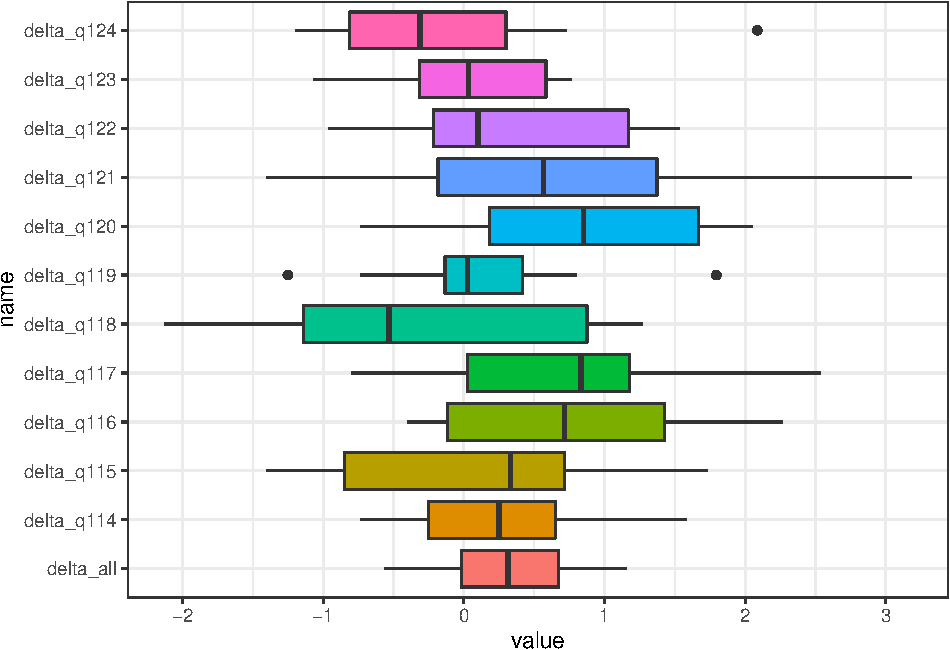
\includegraphics{preanalysis_files/figure-latex/unnamed-chunk-18-1.pdf}

\hypertarget{population-pressure}{%
\subsection{Population pressure}\label{population-pressure}}

\begin{itemize}
\tightlist
\item
  {[}39{]} ``x125\_buildroads\_accessmarkets''\\
\item
  {[}40{]} ``x126\_government\_morebridges''\\
\item
  {[}41{]} ``x127\_government\_raisenarrowbridges''\\
\item
  {[}42{]} ``x128\_newbuildings\_highfloors''\\
\item
  {[}43{]} ``x129\_communities\_ladders''\\
\item
  {[}44{]} ``x130\_government\_oneclassschools''\\
\item
  {[}45{]} ``x131\_commties\_girlsandboys''\\
\item
  {[}46{]} ``x132\_commties\_technicalschools''\\
\item
  {[}47{]} ``x133\_government\_enforceminimumageof18''\\
\item
  {[}48{]} ``x134\_resources\_planningsizeoffamilies''\\
\item
  {[}49{]} ``x135\_education\_familyplanning''\\
\item
  {[}50{]} ``x136\_healthcenter\_i\_is''\\
\item
  {[}51{]} ``x137\_moreroads\_fewerbridges''
\end{itemize}

Again, there's quite a bit of variation. But I'll still keep all of the
questions.

\begin{longtable}[]{@{}rrrrrrrrrrrrrr@{}}
\toprule
\begin{minipage}[b]{0.05\columnwidth}\raggedleft
delta\_q125\strut
\end{minipage} & \begin{minipage}[b]{0.05\columnwidth}\raggedleft
delta\_q126\strut
\end{minipage} & \begin{minipage}[b]{0.05\columnwidth}\raggedleft
delta\_q127\strut
\end{minipage} & \begin{minipage}[b]{0.05\columnwidth}\raggedleft
delta\_q128\strut
\end{minipage} & \begin{minipage}[b]{0.05\columnwidth}\raggedleft
delta\_q129\strut
\end{minipage} & \begin{minipage}[b]{0.05\columnwidth}\raggedleft
delta\_q130\strut
\end{minipage} & \begin{minipage}[b]{0.05\columnwidth}\raggedleft
delta\_q131\strut
\end{minipage} & \begin{minipage}[b]{0.05\columnwidth}\raggedleft
delta\_q132\strut
\end{minipage} & \begin{minipage}[b]{0.05\columnwidth}\raggedleft
delta\_q133\strut
\end{minipage} & \begin{minipage}[b]{0.05\columnwidth}\raggedleft
delta\_q134\strut
\end{minipage} & \begin{minipage}[b]{0.05\columnwidth}\raggedleft
delta\_q135\strut
\end{minipage} & \begin{minipage}[b]{0.05\columnwidth}\raggedleft
delta\_q136\strut
\end{minipage} & \begin{minipage}[b]{0.05\columnwidth}\raggedleft
delta\_q137\strut
\end{minipage} & \begin{minipage}[b]{0.04\columnwidth}\raggedleft
delta\_all\strut
\end{minipage}\tabularnewline
\midrule
\endhead
\begin{minipage}[t]{0.05\columnwidth}\raggedleft
0.120225\strut
\end{minipage} & \begin{minipage}[t]{0.05\columnwidth}\raggedleft
0.0599686\strut
\end{minipage} & \begin{minipage}[t]{0.05\columnwidth}\raggedleft
0.5150576\strut
\end{minipage} & \begin{minipage}[t]{0.05\columnwidth}\raggedleft
0.3412088\strut
\end{minipage} & \begin{minipage}[t]{0.05\columnwidth}\raggedleft
0.5399922\strut
\end{minipage} & \begin{minipage}[t]{0.05\columnwidth}\raggedleft
-0.267831\strut
\end{minipage} & \begin{minipage}[t]{0.05\columnwidth}\raggedleft
0.0999869\strut
\end{minipage} & \begin{minipage}[t]{0.05\columnwidth}\raggedleft
-0.0402407\strut
\end{minipage} & \begin{minipage}[t]{0.05\columnwidth}\raggedleft
0.1973705\strut
\end{minipage} & \begin{minipage}[t]{0.05\columnwidth}\raggedleft
0.5602172\strut
\end{minipage} & \begin{minipage}[t]{0.05\columnwidth}\raggedleft
-0.0575877\strut
\end{minipage} & \begin{minipage}[t]{0.05\columnwidth}\raggedleft
-0.379932\strut
\end{minipage} & \begin{minipage}[t]{0.05\columnwidth}\raggedleft
0.174045\strut
\end{minipage} & \begin{minipage}[t]{0.04\columnwidth}\raggedleft
0.1432677\strut
\end{minipage}\tabularnewline
\bottomrule
\end{longtable}

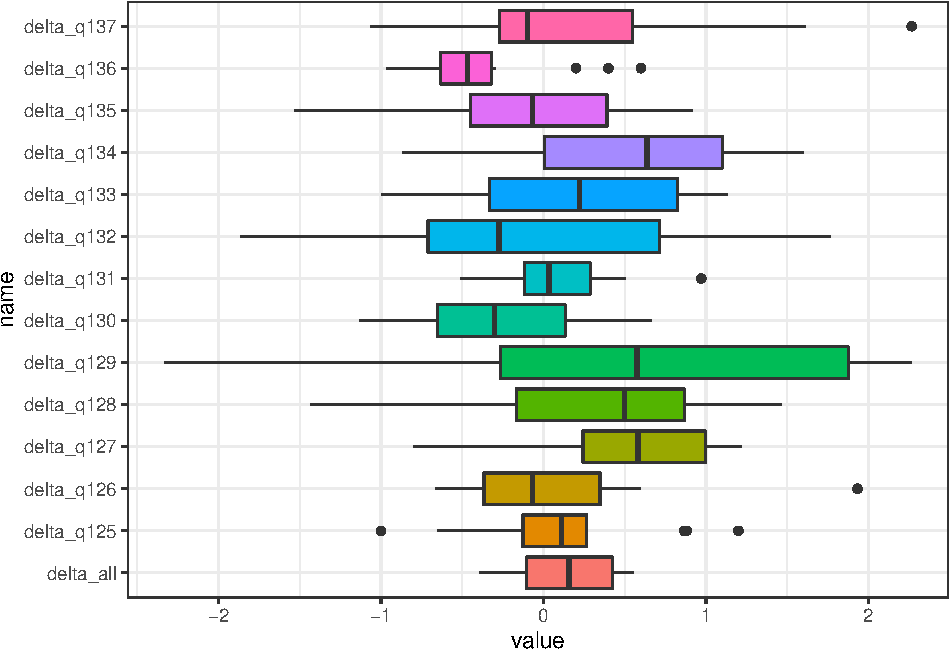
\includegraphics{preanalysis_files/figure-latex/unnamed-chunk-23-1.pdf}

\hypertarget{resettlement}{%
\subsection{Resettlement}\label{resettlement}}

\begin{itemize}
\tightlist
\item
  {[}15{]} ``x101\_rezoning''\\
\item
  {[}16{]} ``x102\_compesation''\\
\item
  {[}17{]} ``x103\_resettle\_hostfamilies''\\
\item
  {[}18{]} ``x104\_support\_hostfamilies''\\
\item
  {[}19{]} ``x105\_strengthen\_dm\_cs''\\
\item
  {[}20{]} ``x106\_raisefunds\_dm\_cs''\\
\item
  {[}21{]} ``x107\_training\_dm\_cs''\\
\item
  {[}22{]} ``x108\_buildperi\_urbancenterrs''\\
\item
  {[}23{]} ``x109\_newperi\_urbancenters\_nearby''
\end{itemize}

Again, there's quite a bit of variation. But I'll still keep all of the
questions.

\begin{longtable}[]{@{}rrrrrrrrrr@{}}
\toprule
\begin{minipage}[b]{0.07\columnwidth}\raggedleft
delta\_q101\strut
\end{minipage} & \begin{minipage}[b]{0.07\columnwidth}\raggedleft
delta\_q102\strut
\end{minipage} & \begin{minipage}[b]{0.07\columnwidth}\raggedleft
delta\_q103\strut
\end{minipage} & \begin{minipage}[b]{0.07\columnwidth}\raggedleft
delta\_q104\strut
\end{minipage} & \begin{minipage}[b]{0.07\columnwidth}\raggedleft
delta\_q105\strut
\end{minipage} & \begin{minipage}[b]{0.07\columnwidth}\raggedleft
delta\_q106\strut
\end{minipage} & \begin{minipage}[b]{0.07\columnwidth}\raggedleft
delta\_q107\strut
\end{minipage} & \begin{minipage}[b]{0.07\columnwidth}\raggedleft
delta\_q108\strut
\end{minipage} & \begin{minipage}[b]{0.07\columnwidth}\raggedleft
delta\_q109\strut
\end{minipage} & \begin{minipage}[b]{0.07\columnwidth}\raggedleft
delta\_all\strut
\end{minipage}\tabularnewline
\midrule
\endhead
\begin{minipage}[t]{0.07\columnwidth}\raggedleft
0.7606881\strut
\end{minipage} & \begin{minipage}[t]{0.07\columnwidth}\raggedleft
-0.1995029\strut
\end{minipage} & \begin{minipage}[t]{0.07\columnwidth}\raggedleft
0.272449\strut
\end{minipage} & \begin{minipage}[t]{0.07\columnwidth}\raggedleft
0.7472135\strut
\end{minipage} & \begin{minipage}[t]{0.07\columnwidth}\raggedleft
0.7106096\strut
\end{minipage} & \begin{minipage}[t]{0.07\columnwidth}\raggedleft
1.145513\strut
\end{minipage} & \begin{minipage}[t]{0.07\columnwidth}\raggedleft
0.3004317\strut
\end{minipage} & \begin{minipage}[t]{0.07\columnwidth}\raggedleft
0.6293694\strut
\end{minipage} & \begin{minipage}[t]{0.07\columnwidth}\raggedleft
0.4556253\strut
\end{minipage} & \begin{minipage}[t]{0.07\columnwidth}\raggedleft
0.5358219\strut
\end{minipage}\tabularnewline
\bottomrule
\end{longtable}

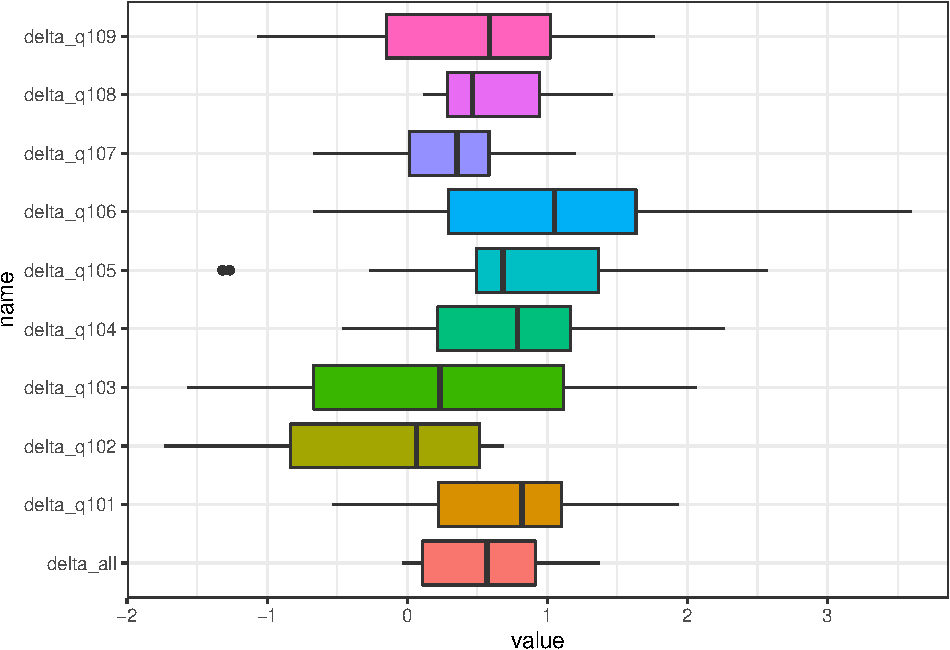
\includegraphics{preanalysis_files/figure-latex/unnamed-chunk-28-1.pdf}

\hypertarget{butaleja}{%
\section{Butaleja}\label{butaleja}}

\hypertarget{land-management-1}{%
\subsection{Land Management}\label{land-management-1}}

\begin{itemize}
\tightlist
\item
  {[}28{]} ``x114\_planttrees\_protectriverbeds''\\
\item
  {[}29{]} ``x115\_riverchannels\_localgovernment''\\
\item
  {[}30{]} ``x116\_wetlands\_dryseason''\\
\item
  {[}31{]} ``x117\_riceschemes\_notinwetlands''\\
\item
  {[}32{]} ``x118\_communities\_maintainwaterchannels''\\
\item
  {[}33{]} ``x119\_communities\_benefitscropdiversity''\\
\item
  {[}34{]} ``x120\_communities\_de\_silting''\\
\item
  {[}35{]} ``x121\_government\_assistdesilting''\\
\item
  {[}36{]} ``x122\_communities\_sanitationdrains''\\
\item
  {[}37{]} ``x123\_government\_drillingcleanwater''\\
\item
  {[}38{]} ``x124\_communities\_resourcesaccesswater''
\end{itemize}

There's quite a bit of variation across questions. However, it all seems
to average out in the ``delta\_all''. So, I'll keep them all for now.

\begin{longtable}[]{@{}rrrrrrrrrrrr@{}}
\toprule
\begin{minipage}[b]{0.06\columnwidth}\raggedleft
delta\_q114\strut
\end{minipage} & \begin{minipage}[b]{0.06\columnwidth}\raggedleft
delta\_q115\strut
\end{minipage} & \begin{minipage}[b]{0.06\columnwidth}\raggedleft
delta\_q116\strut
\end{minipage} & \begin{minipage}[b]{0.06\columnwidth}\raggedleft
delta\_q117\strut
\end{minipage} & \begin{minipage}[b]{0.06\columnwidth}\raggedleft
delta\_q118\strut
\end{minipage} & \begin{minipage}[b]{0.06\columnwidth}\raggedleft
delta\_q119\strut
\end{minipage} & \begin{minipage}[b]{0.06\columnwidth}\raggedleft
delta\_q120\strut
\end{minipage} & \begin{minipage}[b]{0.06\columnwidth}\raggedleft
delta\_q121\strut
\end{minipage} & \begin{minipage}[b]{0.06\columnwidth}\raggedleft
delta\_q122\strut
\end{minipage} & \begin{minipage}[b]{0.06\columnwidth}\raggedleft
delta\_q123\strut
\end{minipage} & \begin{minipage}[b]{0.06\columnwidth}\raggedleft
delta\_q124\strut
\end{minipage} & \begin{minipage}[b]{0.06\columnwidth}\raggedleft
delta\_all\strut
\end{minipage}\tabularnewline
\midrule
\endhead
\begin{minipage}[t]{0.06\columnwidth}\raggedleft
0.4618465\strut
\end{minipage} & \begin{minipage}[t]{0.06\columnwidth}\raggedleft
0.0623585\strut
\end{minipage} & \begin{minipage}[t]{0.06\columnwidth}\raggedleft
0.513398\strut
\end{minipage} & \begin{minipage}[t]{0.06\columnwidth}\raggedleft
-0.4040765\strut
\end{minipage} & \begin{minipage}[t]{0.06\columnwidth}\raggedleft
-0.943491\strut
\end{minipage} & \begin{minipage}[t]{0.06\columnwidth}\raggedleft
0.1775008\strut
\end{minipage} & \begin{minipage}[t]{0.06\columnwidth}\raggedleft
-0.7936031\strut
\end{minipage} & \begin{minipage}[t]{0.06\columnwidth}\raggedleft
0.3935667\strut
\end{minipage} & \begin{minipage}[t]{0.06\columnwidth}\raggedleft
-0.1689441\strut
\end{minipage} & \begin{minipage}[t]{0.06\columnwidth}\raggedleft
0.1475283\strut
\end{minipage} & \begin{minipage}[t]{0.06\columnwidth}\raggedleft
-0.0206571\strut
\end{minipage} & \begin{minipage}[t]{0.06\columnwidth}\raggedleft
-0.0426845\strut
\end{minipage}\tabularnewline
\bottomrule
\end{longtable}

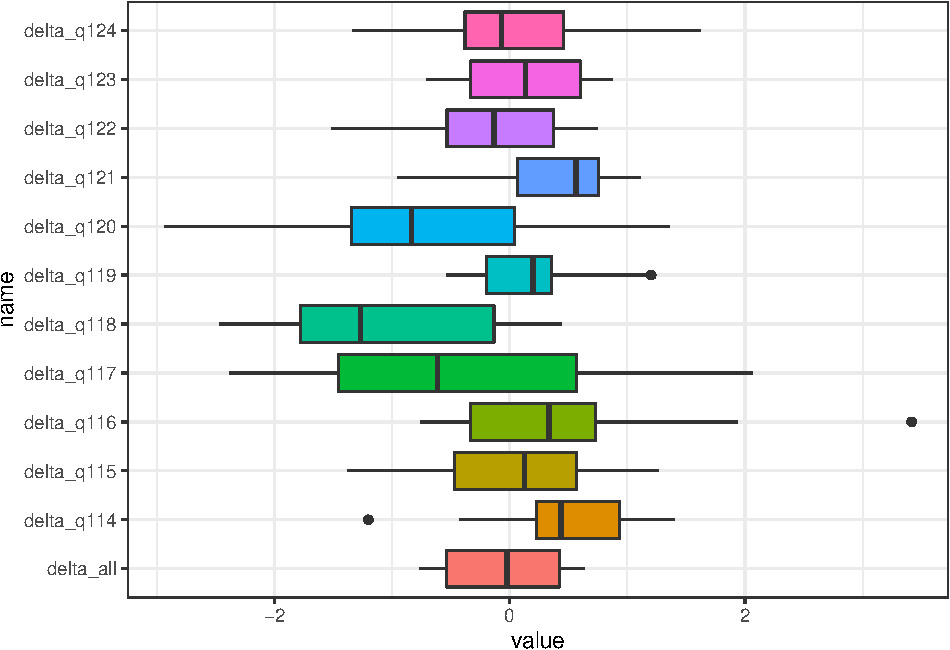
\includegraphics{preanalysis_files/figure-latex/unnamed-chunk-34-1.pdf}

\hypertarget{population-pressure-1}{%
\subsection{Population Pressure}\label{population-pressure-1}}

\begin{itemize}
\tightlist
\item
  {[}39{]} ``x125\_buildroads\_accessmarkets''\\
\item
  {[}40{]} ``x126\_government\_morebridges''\\
\item
  {[}41{]} ``x127\_government\_raisenarrowbridges''\\
\item
  {[}42{]} ``x128\_newbuildings\_highfloors''\\
\item
  {[}43{]} ``x129\_communities\_ladders''\\
\item
  {[}44{]} ``x130\_government\_oneclassschools''\\
\item
  {[}45{]} ``x131\_commties\_girlsandboys''\\
\item
  {[}46{]} ``x132\_commties\_technicalschools''\\
\item
  {[}47{]} ``x133\_government\_enforceminimumageof18''\\
\item
  {[}48{]} ``x134\_resources\_planningsizeoffamilies''\\
\item
  {[}49{]} ``x135\_education\_familyplanning''\\
\item
  {[}50{]} ``x136\_healthcenter\_i\_is''\\
\item
  {[}51{]} ``x137\_moreroads\_fewerbridges''
\end{itemize}

Again, there's quite a bit of variation. I'm going to remove 137 since
it's such an outlier.

\begin{longtable}[]{@{}rrrrrrrrrrrrrr@{}}
\toprule
\begin{minipage}[b]{0.05\columnwidth}\raggedleft
delta\_q125\strut
\end{minipage} & \begin{minipage}[b]{0.05\columnwidth}\raggedleft
delta\_q126\strut
\end{minipage} & \begin{minipage}[b]{0.05\columnwidth}\raggedleft
delta\_q127\strut
\end{minipage} & \begin{minipage}[b]{0.05\columnwidth}\raggedleft
delta\_q128\strut
\end{minipage} & \begin{minipage}[b]{0.05\columnwidth}\raggedleft
delta\_q129\strut
\end{minipage} & \begin{minipage}[b]{0.05\columnwidth}\raggedleft
delta\_q130\strut
\end{minipage} & \begin{minipage}[b]{0.05\columnwidth}\raggedleft
delta\_q131\strut
\end{minipage} & \begin{minipage}[b]{0.05\columnwidth}\raggedleft
delta\_q132\strut
\end{minipage} & \begin{minipage}[b]{0.05\columnwidth}\raggedleft
delta\_q133\strut
\end{minipage} & \begin{minipage}[b]{0.05\columnwidth}\raggedleft
delta\_q134\strut
\end{minipage} & \begin{minipage}[b]{0.05\columnwidth}\raggedleft
delta\_q135\strut
\end{minipage} & \begin{minipage}[b]{0.05\columnwidth}\raggedleft
delta\_q136\strut
\end{minipage} & \begin{minipage}[b]{0.05\columnwidth}\raggedleft
delta\_q137\strut
\end{minipage} & \begin{minipage}[b]{0.05\columnwidth}\raggedleft
delta\_all\strut
\end{minipage}\tabularnewline
\midrule
\endhead
\begin{minipage}[t]{0.05\columnwidth}\raggedleft
-0.1303527\strut
\end{minipage} & \begin{minipage}[t]{0.05\columnwidth}\raggedleft
0.0082831\strut
\end{minipage} & \begin{minipage}[t]{0.05\columnwidth}\raggedleft
-0.0006727\strut
\end{minipage} & \begin{minipage}[t]{0.05\columnwidth}\raggedleft
-0.1042372\strut
\end{minipage} & \begin{minipage}[t]{0.05\columnwidth}\raggedleft
0.1182781\strut
\end{minipage} & \begin{minipage}[t]{0.05\columnwidth}\raggedleft
-0.1985573\strut
\end{minipage} & \begin{minipage}[t]{0.05\columnwidth}\raggedleft
-0.0789363\strut
\end{minipage} & \begin{minipage}[t]{0.05\columnwidth}\raggedleft
-0.363285\strut
\end{minipage} & \begin{minipage}[t]{0.05\columnwidth}\raggedleft
0.4393448\strut
\end{minipage} & \begin{minipage}[t]{0.05\columnwidth}\raggedleft
0.056784\strut
\end{minipage} & \begin{minipage}[t]{0.05\columnwidth}\raggedleft
0.2450377\strut
\end{minipage} & \begin{minipage}[t]{0.05\columnwidth}\raggedleft
-0.0839075\strut
\end{minipage} & \begin{minipage}[t]{0.05\columnwidth}\raggedleft
-1.521286\strut
\end{minipage} & \begin{minipage}[t]{0.05\columnwidth}\raggedleft
-0.1241159\strut
\end{minipage}\tabularnewline
\bottomrule
\end{longtable}

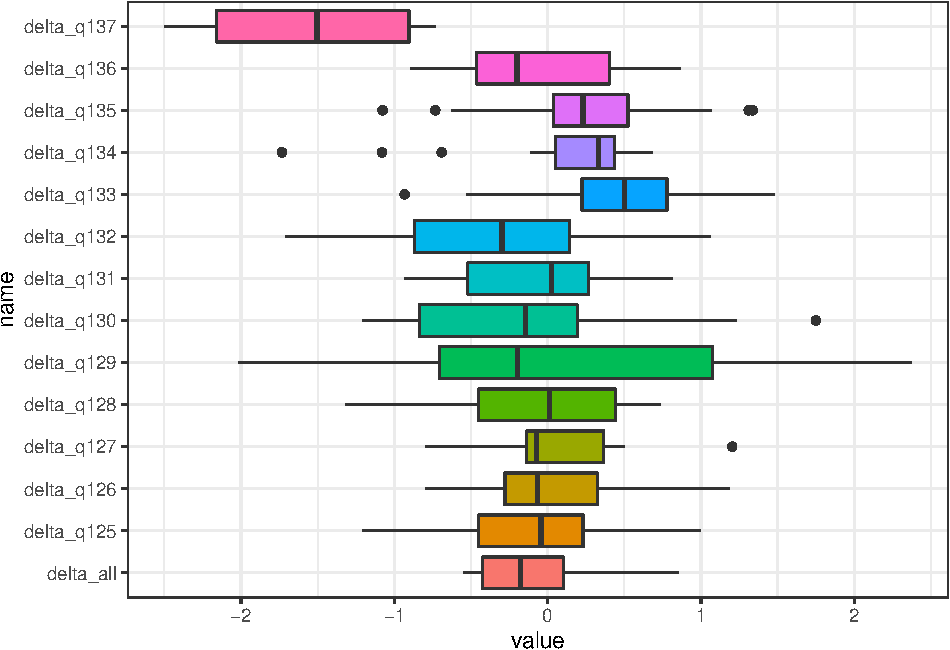
\includegraphics{preanalysis_files/figure-latex/unnamed-chunk-39-1.pdf}

\hypertarget{resettlement-1}{%
\subsection{Resettlement}\label{resettlement-1}}

\begin{itemize}
\tightlist
\item
  {[}15{]} ``x101\_rezoning''\\
\item
  {[}16{]} ``x102\_compesation''\\
\item
  {[}17{]} ``x103\_resettle\_hostfamilies''\\
\item
  {[}18{]} ``x104\_support\_hostfamilies''\\
\item
  {[}19{]} ``x105\_strengthen\_dm\_cs''\\
\item
  {[}20{]} ``x106\_raisefunds\_dm\_cs''\\
\item
  {[}21{]} ``x107\_training\_dm\_cs''\\
\item
  {[}22{]} ``x108\_buildperi\_urbancenterrs''\\
\item
  {[}23{]} ``x109\_newperi\_urbancenters\_nearby''
\end{itemize}

Again, there's quite a bit of variation. I \emph{could} remove 101, but
I'll keep it for now.

\begin{longtable}[]{@{}rrrrrrrrrr@{}}
\toprule
\begin{minipage}[b]{0.07\columnwidth}\raggedleft
delta\_q101\strut
\end{minipage} & \begin{minipage}[b]{0.07\columnwidth}\raggedleft
delta\_q102\strut
\end{minipage} & \begin{minipage}[b]{0.07\columnwidth}\raggedleft
delta\_q103\strut
\end{minipage} & \begin{minipage}[b]{0.07\columnwidth}\raggedleft
delta\_q104\strut
\end{minipage} & \begin{minipage}[b]{0.07\columnwidth}\raggedleft
delta\_q105\strut
\end{minipage} & \begin{minipage}[b]{0.07\columnwidth}\raggedleft
delta\_q106\strut
\end{minipage} & \begin{minipage}[b]{0.07\columnwidth}\raggedleft
delta\_q107\strut
\end{minipage} & \begin{minipage}[b]{0.07\columnwidth}\raggedleft
delta\_q108\strut
\end{minipage} & \begin{minipage}[b]{0.07\columnwidth}\raggedleft
delta\_q109\strut
\end{minipage} & \begin{minipage}[b]{0.07\columnwidth}\raggedleft
delta\_all\strut
\end{minipage}\tabularnewline
\midrule
\endhead
\begin{minipage}[t]{0.07\columnwidth}\raggedleft
1.246048\strut
\end{minipage} & \begin{minipage}[t]{0.07\columnwidth}\raggedleft
0.0403275\strut
\end{minipage} & \begin{minipage}[t]{0.07\columnwidth}\raggedleft
0.6443898\strut
\end{minipage} & \begin{minipage}[t]{0.07\columnwidth}\raggedleft
0.056763\strut
\end{minipage} & \begin{minipage}[t]{0.07\columnwidth}\raggedleft
0.2345946\strut
\end{minipage} & \begin{minipage}[t]{0.07\columnwidth}\raggedleft
-0.0191714\strut
\end{minipage} & \begin{minipage}[t]{0.07\columnwidth}\raggedleft
0.2014177\strut
\end{minipage} & \begin{minipage}[t]{0.07\columnwidth}\raggedleft
-0.2040673\strut
\end{minipage} & \begin{minipage}[t]{0.07\columnwidth}\raggedleft
0.1074079\strut
\end{minipage} & \begin{minipage}[t]{0.07\columnwidth}\raggedleft
0.2564122\strut
\end{minipage}\tabularnewline
\bottomrule
\end{longtable}

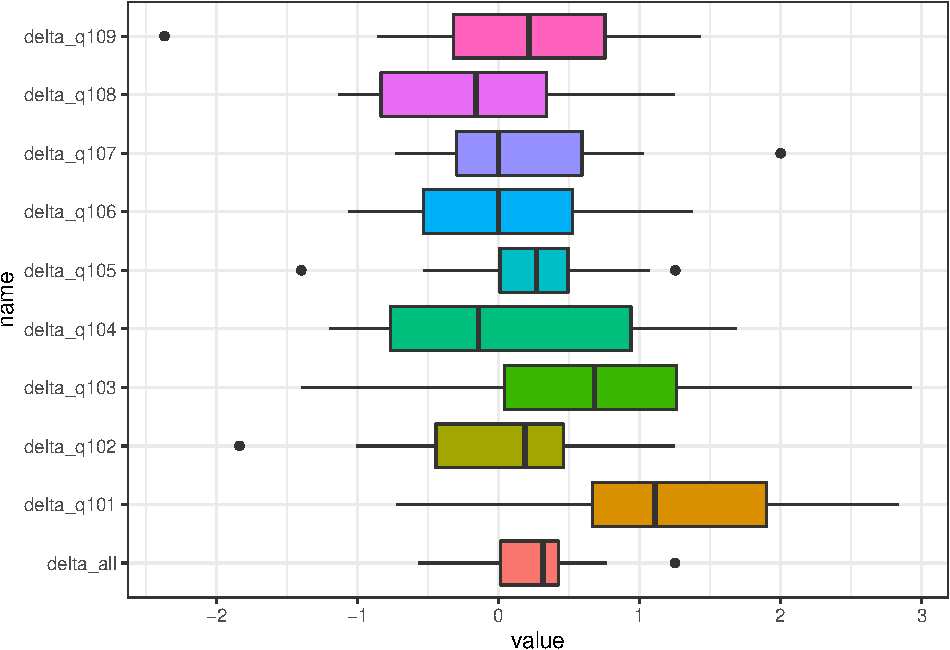
\includegraphics{preanalysis_files/figure-latex/unnamed-chunk-44-1.pdf}





\newpage
\singlespacing 
\end{document}
